\documentclass[11pt]{article}

\usepackage[margin=1.1in]{geometry}
\usepackage{graphicx}
\usepackage{booktabs}
\usepackage{amsmath}
\usepackage{microtype}
\usepackage[hidelinks]{hyperref}
\usepackage{xcolor}
\usepackage{listings}

\graphicspath{{../analysis/plots/}}

\lstset{basicstyle=\ttfamily\footnotesize, breaklines=true, frame=single, framerule=0.3pt}

\title{\textbf{Queueing the Transformer}\\[4pt]
\large LLM inference as an operations research problem:\\
a validated discrete-event model of batched serving}
\author{Shaan Jain\\ \small\texttt{github.com/Shaandjain/llm-inference-queueing}}
\date{June 2026}

\begin{document}
\maketitle

\begin{abstract}
\noindent
LLM serving systems are queueing systems: requests arrive stochastically, occupy a batched server through distinct prefill and decode phases, and contend for KV-cache memory. I built a discrete-event simulator of batched LLM inference on a deliberately small cost model --- two linear coefficients per phase --- and asked whether it can \emph{predict} a real serving system rather than merely illustrate one. Fitting the model from 40 sequential probe requests and a concurrency sweep against vLLM running Qwen2.5-7B-Instruct on an NVIDIA L4, then replaying held-out Poisson workloads open-loop, the simulator predicted median time-to-first-token within 12\% and, after correcting a systematic error, end-to-end latency percentiles within 6--13\% at both 50\% and 80\% of saturation load. The correction itself is the most transferable finding: a latency intercept fitted over a network conflates per-request overhead with per-iteration GPU time, and charging it as GPU-blocking time inflates predicted tail latency by 37--60\%. Along the way the simulation reproduces the canonical continuous-vs-static batching results and surfaces an under-stated operational fact: busy-time ``utilization'' of a batched LLM server saturates near 100\% at \emph{every} load level, making GPU-busy metrics useless as load signals; decode batch occupancy is the signal that tracks load.
\end{abstract}

\section{Introduction}

When an AI agent feels slow, the bottleneck is usually not the model's intelligence but the serving system's queueing behavior: how requests are batched, when prefill preempts decode, and how much headroom the operator left below saturation. These are classical operations research questions --- arrival processes, service-time distributions, scheduling policies, tail latency --- wearing a GPU costume.

This report does three things:

\begin{enumerate}
  \item \textbf{Models} batched LLM serving as a discrete-event system with a two-phase linear cost model (\S\ref{sec:model}), implementing both iteration-level (continuous) batching in the style of Orca~\cite{orca} and vLLM~\cite{vllm}, and classic request-level (static) batching.
  \item \textbf{Reproduces} the canonical serving results from first principles (\S\ref{sec:sim}): a $\sim$5$\times$ capacity gap between continuous and static batching, the tail-latency hockey stick, and the cost of arrival burstiness --- plus one less commonly plotted fact about utilization metrics.
  \item \textbf{Validates} the simulator against a real deployment (\S\ref{sec:validation}): vLLM 0.11 serving Qwen2.5-7B-Instruct on an NVIDIA L4, with coefficients fitted from cheap probes and accuracy assessed on held-out workloads the fitting never saw. Total GPU cost of the validation protocol: about \$1.
\end{enumerate}

Nothing in \S\ref{sec:sim} is a new result; simulators of LLM serving exist, notably Vidur~\cite{vidur}. The contribution here is methodological and pedagogical: a compact (under 1{,}000 lines), fully open simulator with a fit-predict-attribute validation loop, and two documented measurement traps (\S\ref{sec:traps}) that anyone benchmarking inference over a network will encounter.

\section{Model}\label{sec:model}

\paragraph{Requests.} A request $r$ arrives at time $a_r$ with $p_r$ prompt tokens and $g_r$ tokens to generate. Workload profiles (\texttt{chat}, \texttt{rag}, \texttt{agent}) draw $(p_r, g_r)$ from lognormal distributions; arrivals are Poisson or an on/off bursty process calibrated to the same mean rate.

\paragraph{Server.} The engine executes iterations. A \emph{prefill} iteration processes the prompts of newly admitted requests and emits their first token; a \emph{decode} iteration generates one token for every active sequence. Iteration costs are linear:
\begin{align}
T_{\text{prefill}}(n_{\text{tok}}) &= \beta_p + \kappa_p \, n_{\text{tok}}, &
T_{\text{decode}}(b) &= \beta_d + \kappa_d \, b,
\end{align}
where $n_{\text{tok}}$ is total prompt tokens in the iteration and $b$ is the decode batch size. KV-cache occupancy is bounded by a capacity parameter; admission reserves a request's full footprint $p_r + g_r$.

\paragraph{Schedulers.} \emph{Continuous batching} admits requests between iterations up to a batch-size cap and prefill token budget, prioritizing prefill when admissible work is waiting (vLLM's default disposition). \emph{Static batching} takes up to $B$ requests, prefills them together, and decodes until the longest request finishes; completed sequences pad the batch at full cost.

\paragraph{Simplifications.} The scheduler knows $g_r$ at admission (no preemption is modeled); prefill is never chunked or overlapped with decode; the decode cost ignores KV-length effects ($\kappa_{kv}=0$). \S\ref{sec:validation} quantifies what these simplifications cost.

\section{Simulation findings}\label{sec:sim}

All experiments use 1{,}500-request workloads, 5 seeds, and min--max bands; load is expressed as a fraction of each policy's \emph{measured} saturation throughput so policies are compared fairly. One command regenerates every figure from raw traces.

\subsection{Continuous vs.\ static batching}

On the chat profile, continuous batching saturates at 5.10 requests/s against 1.05 for static batch-8 --- the expected $\sim$5$\times$ gap~\cite{orca,vllm}, here derived from queueing structure alone (Figure~\ref{fig:loadsweep}). Raising the static batch to 32 lifts capacity only to 1.70 rps, still below continuous batching capped at batch 8 (2.18 rps): padding waste does not average out (Figure~\ref{fig:frontier}).

\begin{figure}[t]
  \centering
  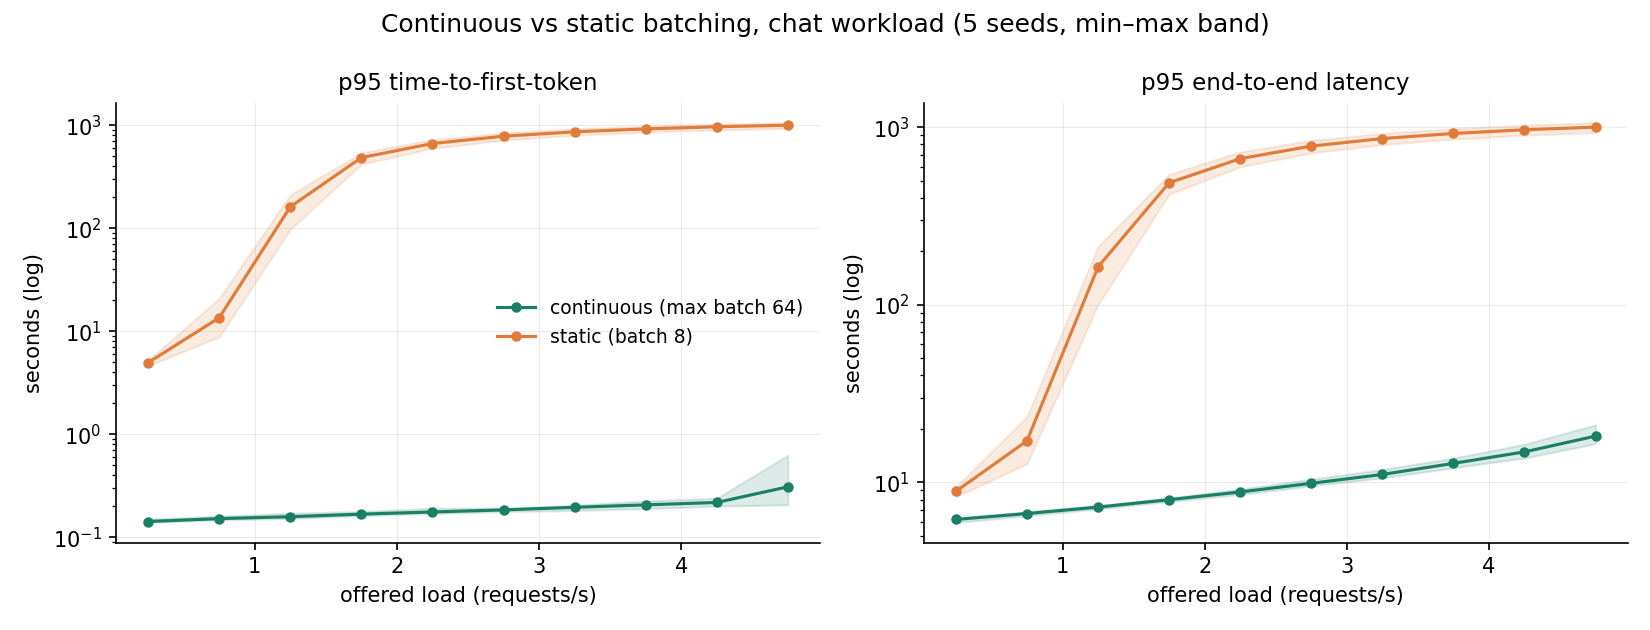
\includegraphics[width=\textwidth]{01_load_sweep.png}
  \caption{p95 TTFT and end-to-end latency vs.\ offered load, chat workload. Static batching's tail explodes past $\sim$1 rps while continuous batching serves 4.75 rps at sub-second p95 TTFT.}
  \label{fig:loadsweep}
\end{figure}

\begin{figure}[t]
  \centering
  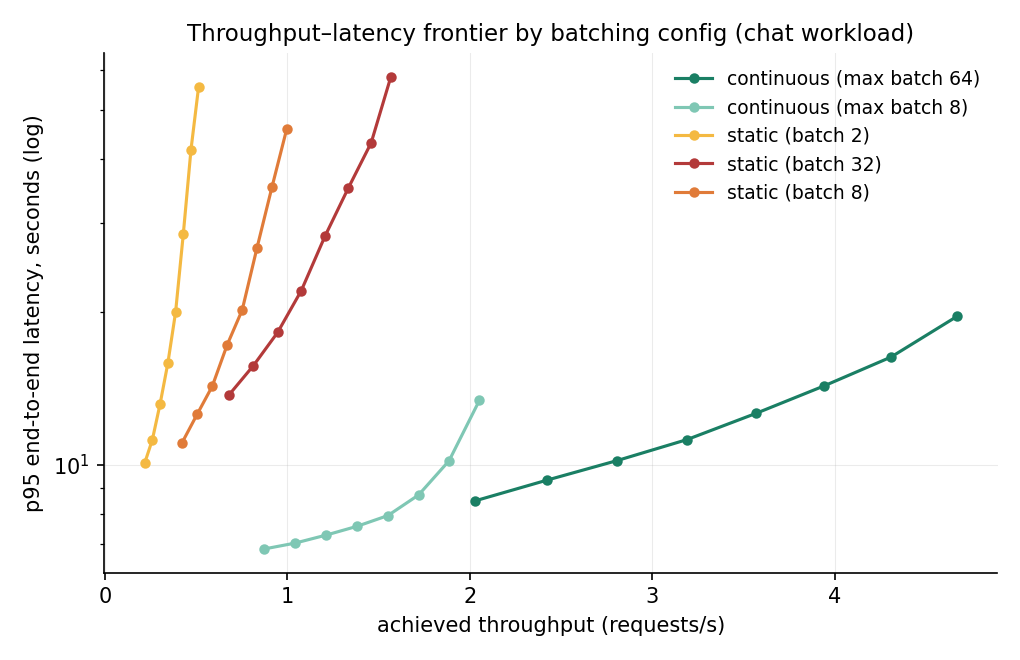
\includegraphics[width=0.72\textwidth]{04_frontier.png}
  \caption{Throughput--latency frontiers by batching configuration. Every static configuration is dominated by continuous batching at any batch cap.}
  \label{fig:frontier}
\end{figure}

\subsection{``Busy'' is not a load signal}

Plotting p95 latency against busy-time utilization produced a degenerate figure: utilization is $\geq 0.97$ at \emph{every} offered load from 30\% to 98\% of capacity. The server never idles --- at low load it simply runs underfilled batches, paying nearly the full per-iteration cost ($\beta_d$ dominates) to produce few tokens. The metric that actually tracks load is decode batch occupancy (Figure~\ref{fig:busy}). Operationally: a dashboard showing ``GPU busy: 99\%'' says nothing about headroom; mean batch occupancy and queue depth do.

\begin{figure}[t]
  \centering
  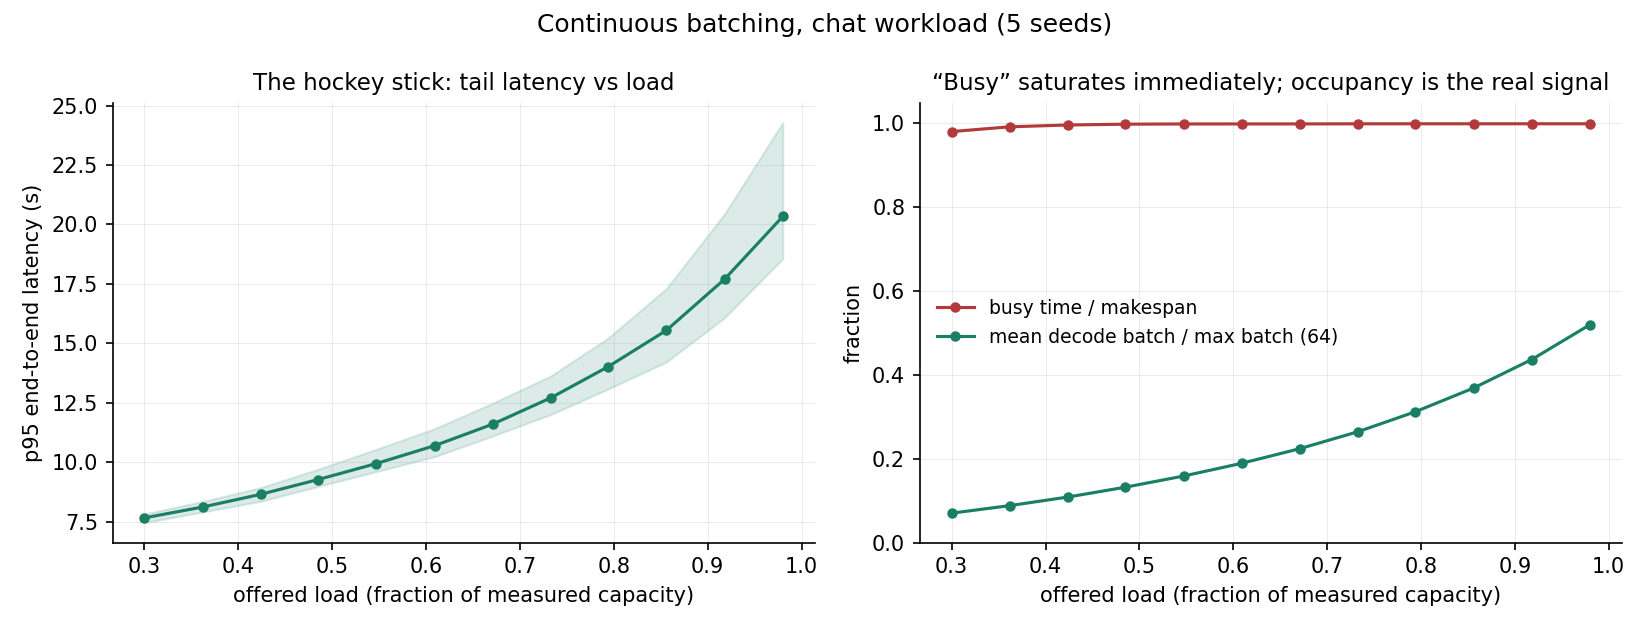
\includegraphics[width=\textwidth]{02_p95_vs_utilization.png}
  \caption{Left: the tail-latency hockey stick vs.\ load. Right: busy-time utilization is flat at $\approx$1.0 across the entire sweep, while batch occupancy rises with load --- occupancy, not busyness, is the real signal.}
  \label{fig:busy}
\end{figure}

\subsection{Burstiness}

At identical mean arrival rates, an on/off arrival process (4$\times$ intensity bursts, 20\% duty cycle) roughly doubles p95 TTFT relative to Poisson across all load levels on the agent profile (Figure~\ref{fig:bursty}). Capacity planning on mean load alone systematically under-provisions for agentic traffic, which is naturally bursty (tool-call fan-outs, retries).

\begin{figure}[t]
  \centering
  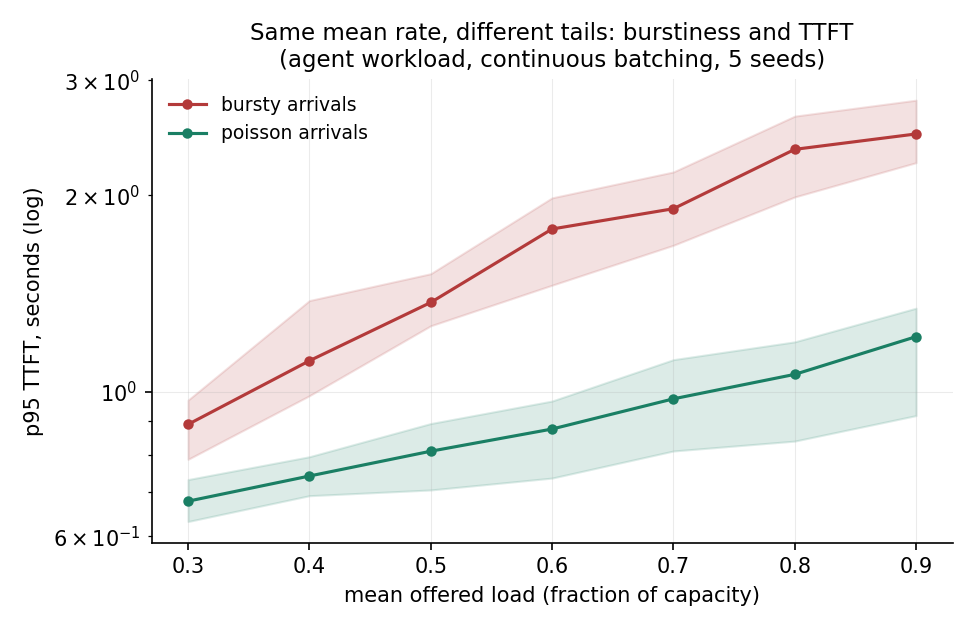
\includegraphics[width=0.62\textwidth]{03_burstiness.png}
  \caption{Same mean rate, different tails: bursty arrivals vs.\ Poisson, agent workload.}
  \label{fig:bursty}
\end{figure}

\section{Validation against vLLM on an L4}\label{sec:validation}

A simulator that only draws plausible curves is decoration. The test: fit the cost model from cheap probes, then predict latency distributions for workloads the fitting never saw.

\subsection{Protocol}

\textbf{Serve.} vLLM 0.11.0, Qwen2.5-7B-Instruct (bf16), NVIDIA L4 on Modal; \texttt{max\_num\_seqs} 64, \texttt{max\_model\_len} 8192. The client runs on a laptop in Toronto; all measurements traverse the public internet, which turns out to matter (\S\ref{sec:attribution}).

\textbf{Fit.} (i) A sequential prompt-length sweep (40 requests, 63--2{,}873 prompt tokens) fits the prefill line: $T_{\text{TTFT}} = 271.6\,\text{ms} + 0.288\,\text{ms/token}$ ($R^2 = 0.887$). (ii) A concurrency sweep ($c \in \{1,2,4,8,16,32\}$, fixed shapes, forced 128-token outputs) fits decode: $T_{\text{TPOT}} = 56.9\,\text{ms} + 0.67\,\text{ms/seq}$ ($R^2 = 0.702$). Batching is nearly free up to $c{=}16$ (58.7\,ms $\to$ 66\,ms per token) --- the measured economics behind \S\ref{sec:sim}.

\textbf{Predict and replay.} The fitted simulator predicts L4 saturation at 1.46 rps on the chat profile. Two held-out Poisson workloads (250 requests each, unseen seeds) were replayed open-loop at 0.73 and 1.17 rps --- 50\% and 80\% of predicted capacity --- with exact output lengths forced via \texttt{ignore\_eos} so simulator and server process identical request sets. Maximum dispatch lag was 18\,ms, so the intended arrival process survived contact with the event loop.

\subsection{Results and error attribution}\label{sec:attribution}

\begin{table}[h]
\centering
\small
\begin{tabular}{llrrrr}
\toprule
Model variant & Load & p50 TTFT & p95 TTFT & p50 e2e & p95 e2e \\
\midrule
raw fit & 0.73 rps & $-12\%$ & $-7\%$ & $+37\%$ & $+41\%$ \\
raw fit & 1.17 rps & $-10\%$ & $-3\%$ & $+60\%$ & $+51\%$ \\
overhead-attributed & 0.73 rps & $-15\%$ & $-33\%$ & $\mathbf{+6\%}$ & $\mathbf{+9\%}$ \\
overhead-attributed & 1.17 rps & $-15\%$ & $-33\%$ & $\mathbf{+13\%}$ & $\mathbf{+11\%}$ \\
\bottomrule
\end{tabular}
\caption{Prediction error (predicted vs.\ observed percentiles, $n{=}250$ per run). Observed values at 1.17 rps: p50/p95 TTFT 0.45/0.72\,s; p50/p95 e2e 9.6/35.2\,s.}
\label{tab:validation}
\end{table}

The raw fitted model nails TTFT but overpredicts end-to-end latency by 37--60\% (Table~\ref{tab:validation}). The cause is an attribution error, not a noise problem. The 272\,ms prefill intercept is dominated by \emph{per-request} overhead --- network round trips, API processing, tokenization, scheduling delay --- but the simulator charges $\beta_p$ on every prefill \emph{iteration} as GPU-blocking time during which all decodes stall. Real vLLM overlaps chunked prefill with decode, and a network round trip blocks nobody's decode. At 0.73 rps over a 354\,s window, the phantom serialized time is roughly $258 \times 240\,\text{ms} \approx 62\,\text{s}$ of fictitious server busyness.

Re-running the prediction with 240\,ms of the intercept reattributed as non-blocking per-request overhead collapses e2e error to $+6$--$13\%$ at both load levels (Figure~\ref{fig:validation}); the predicted and observed e2e CDFs nearly coincide. The correction is not free: a constant offset cannot model TTFT \emph{variance}, so predicted TTFT tails become too tight ($-33\%$ at p95). A proper treatment would fit per-request overhead as a distribution and model chunked prefill; both are future work.

\begin{figure}[t]
  \centering
  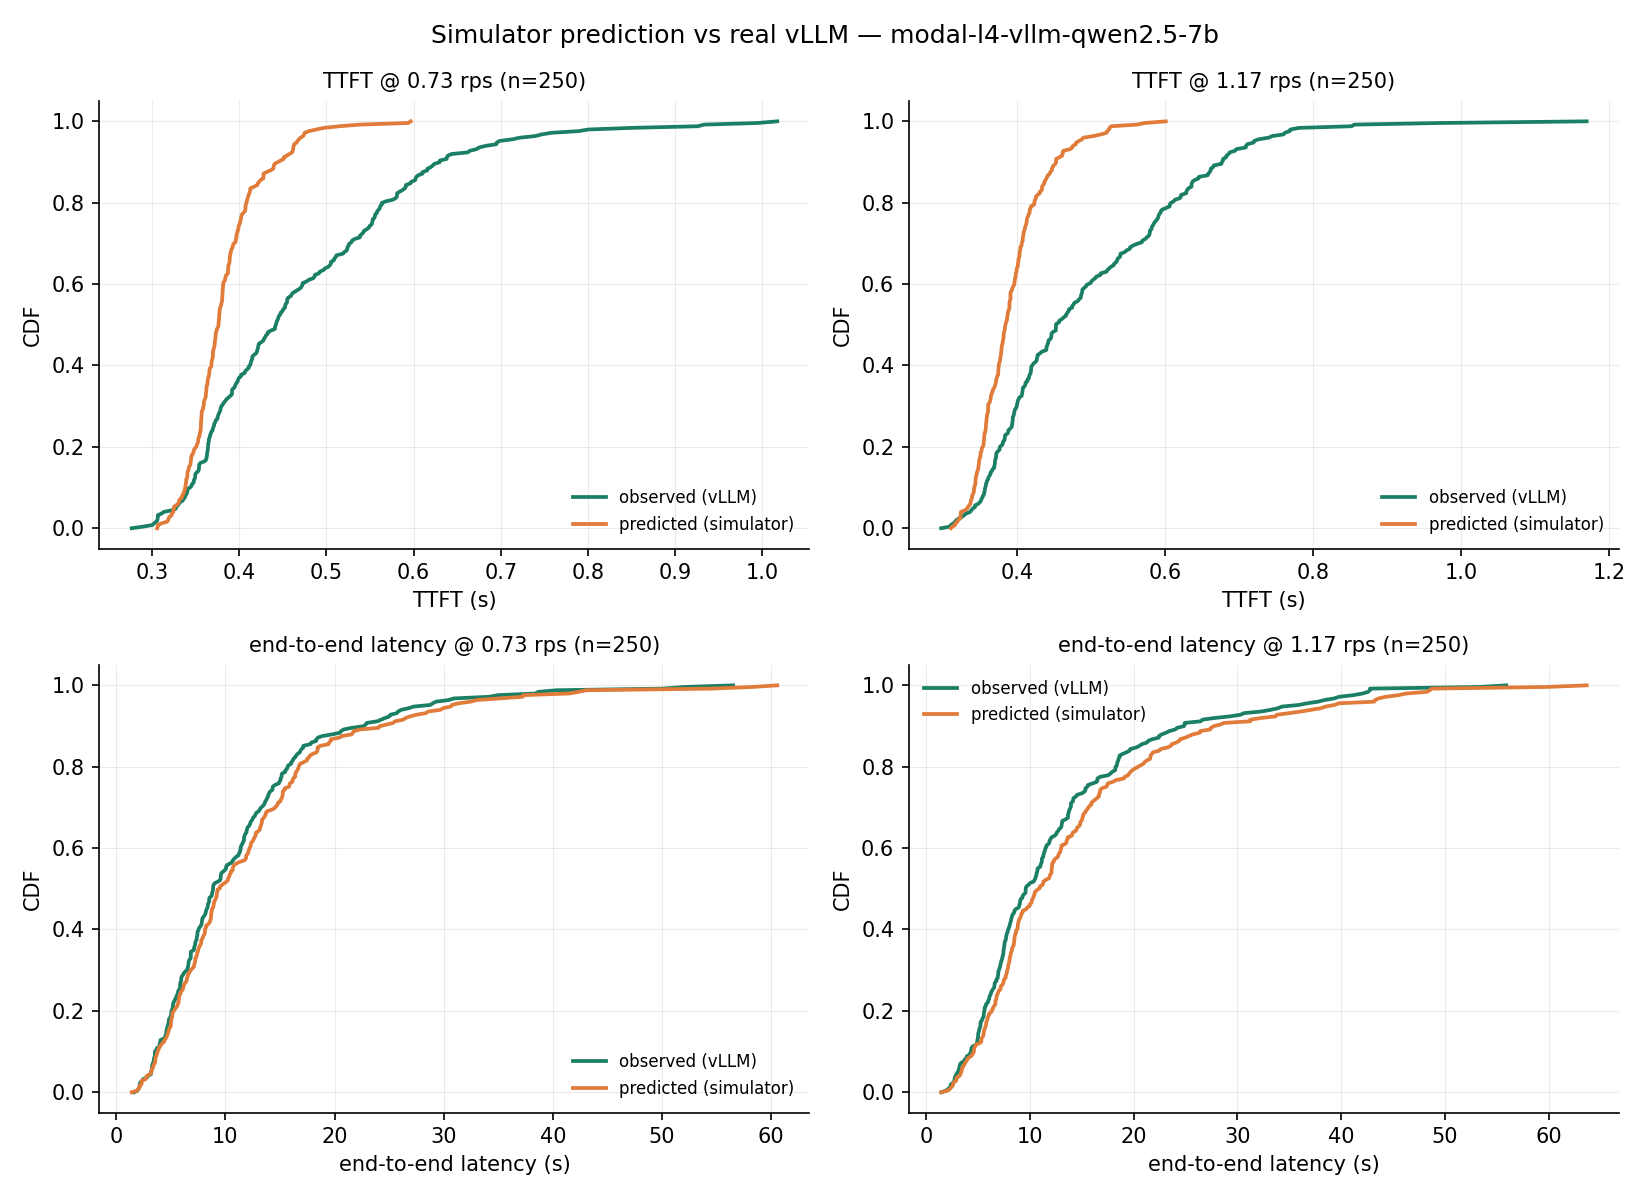
\includegraphics[width=\textwidth]{05_validation_overhead-ablation.png}
  \caption{Predicted vs.\ observed CDFs after overhead attribution, both replay loads. Bottom row: end-to-end latency distributions nearly coincide. Top row: predicted TTFT is correct in location but under-dispersed.}
  \label{fig:validation}
\end{figure}

\section{Measurement traps}\label{sec:traps}

Two failure modes consumed real debugging time and generalize to any inference benchmarking effort.

\paragraph{Prefix caching invalidates repeated prompts.} An earlier fitting run against a local Ollama server (qwen2.5:3b, Apple M3~Pro) produced repetitions with flat 0.13\,s TTFT regardless of prompt length, against 5.6\,s cold at 2{,}834 tokens: the server's prompt cache skipped prefill for identical prompts, so three of four ``repetitions'' measured the cache. Servers cache by longest matching prefix; the fix is a unique nonce at the \emph{start} of every benchmark prompt. (With caching defeated, the same protocol fit the M3~Pro cleanly: $10.2\,\text{ms} + 1.925\,\text{ms/token}$, $R^2 = 0.999$.)

\paragraph{Fitted intercepts conflate overhead classes.} As \S\ref{sec:attribution} shows, a latency intercept fitted over a network bundles per-request costs with per-iteration GPU costs. Any model that serializes the former across concurrent work will overpredict latency under load --- by 37--60\% in this setup. Separating the classes requires either server-side timing or an explicit overhead term; assuming the split is the current method's main internal threat to validity.

\section{Limitations}

The validation covers one model, one GPU, one workload family, two below-saturation load levels, and a single 250-request replay per level. Chunked prefill is not modeled; the 240\,ms overhead split is an ablation estimate rather than an independent measurement; predicted TTFT carries no variance model; KV-length effects on decode cost are disabled; and the simulator's admission control reserves full output length, which real schedulers cannot know. The simulation experiments in \S\ref{sec:sim} use hand-set placeholder coefficients, so their \emph{comparisons} are the claims, not their magnitudes.

\section{Outlook}

The natural next step is to use the queueing frame for what it is good at: deriving operating rules. Heavy-traffic approximations should yield closed-form headroom rules of the form ``for this arrival burstiness and service-time CV, run at $\rho^*$ to hold p95 below $X$'' --- checkable against the L4 traces already collected. On the systems side: chunked-prefill modeling, fitted overhead distributions, and scheduler variants (shortest-prefill-first, deadline-aware) that the simulator can evaluate without renting another GPU.

\appendix

\section{Reproduction}

\begin{lstlisting}
git clone https://github.com/Shaandjain/llm-inference-queueing
uv sync && uv run pytest                       # 10 tests
uv run python experiments/run_experiments.py   # 350 sims (~1 min, CPU)
uv run python analysis/make_plots.py           # figures 1-4
# validation (requires a Modal account; ~$1 of L4 time):
modal deploy serving/vllm_modal.py
uv run python live/capture_traces.py    --base-url <URL>/v1 ...
uv run python live/concurrency_sweep.py --base-url <URL>/v1 ...
uv run python live/fit_coefficients.py  results/l4-prefill \
    --concurrency-dir results/l4-conc --label modal-l4-vllm-qwen2.5-7b
uv run python live/replay_workload.py   --rate 0.73 --seed 42 ...
uv run python analysis/validate.py --request-overhead-s 0.24 ...
modal app stop -y vllm-l4-qwen7b
\end{lstlisting}

All raw traces ship in the repository in a shared JSONL schema; every figure and table regenerates from them.

\section{A note on version skew}

The first deployment failed at server start: vLLM 0.11.0 resolved against transformers 5.x, which removed \texttt{all\_special\_tokens\_extended}. The fix is pinning \texttt{transformers==4.57.1} alongside the vLLM pin. Serving images should pin the full inference stack, not just the engine.

\begin{thebibliography}{9}

\bibitem{orca} G.-I. Yu, J. S. Jeong, G.-W. Kim, S. Kim, and B.-G. Chun. Orca: A distributed serving system for transformer-based generative models. \emph{OSDI}, 2022.

\bibitem{vllm} W. Kwon, Z. Li, S. Zhuang, Y. Sheng, L. Zheng, C. H. Yu, J. Gonzalez, H. Zhang, and I. Stoica. Efficient memory management for large language model serving with PagedAttention. \emph{SOSP}, 2023. arXiv:2309.06180.

\bibitem{vidur} A. Agrawal, N. Kedia, J. Mohan, A. Panwar, N. Kwatra, B. Gulavani, R. Ramjee, and A. Tumanov. Vidur: A large-scale simulation framework for LLM inference. \emph{MLSys}, 2024.

\bibitem{sglang} L. Zheng, L. Yin, Z. Xie, et al. SGLang: Efficient execution of structured language model programs. \emph{NeurIPS}, 2024.

\end{thebibliography}

\end{document}
